\begin{titlingpage}

\newcommand\nbvspace[1][3]{\vspace*{\stretch{#1}}}
% allow some slack to avoid under/overfull boxes
\newcommand\nbstretchyspace{\spaceskip0.5em plus 0.25em minus 0.25em}
% To improve spacing on titlepages
\newcommand{\nbtitlestretch}{\spaceskip0.6em}
\pagestyle{empty}

\begin{center}
\bfseries
\nbvspace[1]

\Large Sheldon Axler.\\
\Huge
{\nbtitlestretch\Huge Álgebra Lineal}\\
\vspace{.5cm}
\large
\nbvspace[1]

RESOLUCIÓN DE PROBLEMAS\\
Y APUNTES\\

\nbvspace[1]
\small POR\\
\Large FODE\\[0.5em]
\footnotesize CHRISTIAN LIMBERT PAREDES AGUILERA\\

\nbvspace[2]

Identidad de Apollonius: $a^2+b^2=\dfrac{1}{2}c^2+2d^2$

\begin{center}
    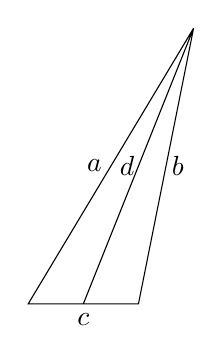
\begin{tikzpicture}[scale=.7]
	\draw[](0,0)node[below]{$c$}--(-1,0)--(2,5)--(0,0)--(1,0)--(2,5);
	\draw[](.2,2.5)node[]{$a$};
	\draw[](1.1,2.5)node[left]{$d$};
	\draw[](2,2.5)node[left]{$b$};
    \end{tikzpicture}
\end{center}

\nbvspace[3]
\normalsize

LIBRO EN SU TERCERA EDICIÓN (Ingles)\\
\large
\nbvspace[1]

\end{center}

\break
\bfseries 

\nbvspace[1]
Título de la obra original:\\
Linear Algebra Done Right\\
Identificadores: \\
ISSN 0172-6056\\
ISBN 978-3-319-11079-0\\
DOI 10.1007/978-3-319-11080-6\\
Springer Cham Heidelberg New York Dordrecht London\\


\nbvspace[1]

\begin{center}
Sin ninguna revisión de esta obra.\\


\nbvspace[1]
    Propiedad de esta obra:\\ 

    CHRISTIAN LIMBERT PAREDES AGUILERA\\	

    E-mail: soyfode@gmail.com
\end{center}

\nbvspace[1]

Reservados todos los derechos. La reproducción total o parcial de esta obra, por cualquier medio o procedimiento, comprendidos la reprografía y el tratamiento informático, y la distribución de ejemplares de ella mediante alquiler o préstamo públicos, queda rigurosamente prohibida sin la autorización escrita de los titulares del copyright, bajo las sanciones establecidas por las leyes.\\

\center 2022 

\end{titlingpage}


\pagenumbering{roman}


\pagestyle{fancy}
\fancyhead[LE,RO]{\nouppercase{\truncate{0.5\headwidth}{\rightmark}}}
\fancyhead[LO,RE]{\nouppercase{\truncate{0.5\headwidth}{\leftmark}}}


